%%%%%%%%%%%%%%%%%%%%%%%%%%%%%%%%%%%%%%%%%
% Journal Article
% LaTeX Template
% Version 1.3 (9/9/13)
%
% This template has been downloaded from:
% http://www.LaTeXTemplates.com
%
% Original author:
% Frits Wenneker (http://www.howtotex.com)
%
% License:
% CC BY-NC-SA 3.0 (http://creativecommons.org/licenses/by-nc-sa/3.0/)
%
%%%%%%%%%%%%%%%%%%%%%%%%%%%%%%%%%%%%%%%%%

%----------------------------------------------------------------------------------------
%	PACKAGES AND OTHER DOCUMENT CONFIGURATIONS
%----------------------------------------------------------------------------------------

\documentclass[twoside]{article}
\usepackage{graphicx}

\usepackage[sc]{mathpazo} % Use the Palatino font
\usepackage[T1]{fontenc} % Use 8-bit encoding that has 256 glyphs
\linespread{1.05} % Line spacing - Palatino needs more space between lines
\usepackage{microtype} % Slightly tweak font spacing for aesthetics

\usepackage[hmarginratio=1:1,top=32mm,columnsep=20pt]{geometry} % Document margins
\usepackage{multicol} % Used for the two-column layout of the document
\usepackage[hang, small,labelfont=bf,up,textfont=it,up]{caption} % Custom captions under/above floats in tables or figures
\usepackage{booktabs} % Horizontal rules in tables
\usepackage{float} % Required for tables and figures in the multi-column environment - they need to be placed in specific locations with the [H] (e.g. \begin{table}[H])
\usepackage{hyperref} % For hyperlinks in the PDF

\usepackage{lettrine} % The lettrine is the first enlarged letter at the beginning of the text
\usepackage{paralist} % Used for the compactitem environment which makes bullet points with less space between them

\usepackage{abstract} % Allows abstract customization
\renewcommand{\abstractnamefont}{\normalfont\bfseries} % Set the "Abstract" text to bold
\renewcommand{\abstracttextfont}{\normalfont\small\itshape} % Set the abstract itself to small italic text

\usepackage{titlesec} % Allows customization of titles
\renewcommand\thesection{\Roman{section}} % Roman numerals for the sections
\renewcommand\thesubsection{\arabic{subsection}} % Roman numerals for subsections
\titleformat{\section}[block]{\large\scshape\centering}{\thesection.}{1em}{} % Change the look of the section titles
\titleformat{\subsection}[block]{\large}{\thesubsection.}{1em}{} % Change the look of the section titles

\usepackage{fancyhdr} % Headers and footers
\pagestyle{fancy} % All pages have headers and footers
\fancyhead{} % Blank out the default header
\fancyfoot{} % Blank out the default footer
\fancyhead[C]{PPGEB - FEELT - UFU $\bullet$ 2013/2} % Custom header text
\fancyfoot[RO,LE]{\thepage} % Custom footer text

\usepackage[utf8]{inputenc}
\usepackage{graphicx}
\graphicspath{{imgs/}}

\usepackage{listings}
\usepackage{xcolor}

\lstdefinestyle{sharpc}{language=[Sharp]C, frame=lr, rulecolor=\color{blue!80!black}, breaklines=true}

%----------------------------------------------------------------------------------------
%	TITLE SECTION
%----------------------------------------------------------------------------------------

\title{\vspace{-15mm}\fontsize{24pt}{10pt}\selectfont\textbf{Algoritmo genético básico para otimização de soluções em um problema de busca do valor máximo de uma função}} % Article title

\author{
\large
\textsc{Daniel Teodoro Gonçalves Mariano, Keiji Yamanaka (Ph.D)}\\[2mm] % Your name
\normalsize Universidade Federal de Uberlândia\\ \normalsize Uberlândia-MG, Brasil \\ % Your institution
\normalsize {dtgmariano@gmail.com, keiji@ufu.br} % Your email address
\vspace{-5mm}
}
\date{}

%----------------------------------------------------------------------------------------

\begin{document}

\maketitle % Insert title

\thispagestyle{fancy} % All pages have headers and footers

%----------------------------------------------------------------------------------------
%	ABSTRACT
%----------------------------------------------------------------------------------------


\begin{abstract}
\noindent
Algoritmo genético é uma heurística de busca que simula o processo de evolução das espécies observado em sistemas biológicos
\end{abstract}

%----------------------------------------------------------------------------------------
%	ARTICLE CONTENTS
%----------------------------------------------------------------------------------------

\begin{multicols}{2} % Two-column layout throughout the main article text

\section{Introduçao}

\subsection{Algoritmos Evolucionários}
Algoritmos evolucionários utilizam modelos computacionais baseados em processos naturais de evolução como um instrumento para a resolução de problemas. Os modelos computacionais propostos se orientam pela simulação de conceitos de evolução das espécies: seleção, mutação e reprodução. Os algoritmos evolucionários operam proporcionando a manutenção de uma população de estruturas, chamadas de indivíduos ou cromossomos. Esses indivíduos se comportam de maneira similar à evolução das espécies, sendo submetidos à operadores genéticos (recombinação e mutação).Cada cromossomo recebe uma avaliação de acordo com o nível de aptidão que este possui dentro do contexto de um problema.

\subsection{Algoritmos Genéticos}
Algoritmos genéticos são um ramo dos algoritmos evolucionários, podendo ser definido como uma técnica de busca baseada numa metáfora do processo biológico de evolução natural. São técnicas heurísticas de otimização global. A otimização global é uma questão que opõe os GAs aos métodos como gradiente (hill climbing), que seguem a derivada de uma função de forma a encontrar o máximo de uma função, ficando facilmente retidos em máximos locais. Nos GAs, populações de indivíduos são criadas e submetidas aos operadores genéticos: seleção, recombinação (crossover) e mutação. Tais operadores utilizam uma caracterização da qualidade de cada individuo como solução do problema em questão chamada de avaliação. Dessa forma geram um processo de evolução natural destes indivíduos, que eventualmente devera gerar um individuo que caracterizara uma boa solução para o nosso problema.

\subsection{Etapas de um AG}
Um AG pode ser dividido nas seguintes etapas:

\begin{enumerate}
\setlength{\itemsep}{0.2cm}%
 \setlength{\parskip}{0.2cm}
\item Inicialização: A população inicial de soluções candidatas são usualmente geradas randomicamente ao longo do espaço de busca. Conhecimentos ou informações específicas do domínio do problema podem ser incorporadas ao algoritmo.
\item Avaliação: Uma vez que a população é iniciada ou uma população descendente é criada, os valores de aptidão das soluções candidatas é avaliada.
\item Seleção: Aloca mais cópias dessas soluções com valores de aptidão superior e, assim, impõe o mecanismo de sobrevivência do mais apto nas soluções candidatas. A idéia principal da seleção é de preferir as melhores soluções em relação as piores.
\item Recombinação: Combina partes de dois ou mais cromossomos (soluções/indivíduos parentais) para gerar um novo cromossomo. Existem diferentes maneiras de se realizar a combinação entre indivíduos. A performance dessa etapa está relacionado com o quão apropriado é o mecanismo de recombinação projetado para aquele contexto. A prole sob recombinação não será idêntico a um pai em particular, pois irá recombinar traços dos pais de uma maneira nova
\item Mutação: Enquanto a recombinação ocorre envolvendo dois ou mais cromossomos a mutação ocorre individualmente. A mutação promove a alteração da solução de maneira randômica. Existem diversas variações de mutações, geralmente envolvendo uma ou mais alterações dos traços de um cromossomo.
\item Reposição: A população criada através da seleção, recombinação e mutação, substituirá os cromossoms pais. 
\item Verificação da condição parada: Enquanto a condição de parada não foi encontrada, repete-se os procedimentos do passo 2 ao 6.
\end{enumerate}

\begin{figure}[H]
  \caption{Diagrama de blocos de um AG básico.}
  \centering
    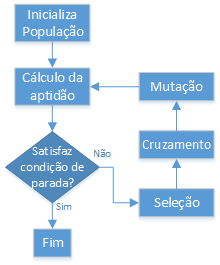
\includegraphics[scale = 1]{basicga_diagram.png}
\end{figure}

%------------------------------------------------

\section{Métodos}
O artigo vigente apresentará os princípios básicos de um algoritmo genético no desenvolvido de uma aplicaçao para minimizar uma funçao multimodal. O software da aplicação foi desenvolvido na plataforma .NET, em linguagem computacional CSharp (C\#).

\begin{equation}
\label{eq:probfunc}
f(x) = x*sin(x/5)
\end{equation}

A função \ref{eq:probfunc} é uma função senoidal, possuindo diversos mínimos e máximos locais. Para o problema foi determinado o domínio [0, 500] para valores que x pode assumir.

\subsection{Representação cromossomial}
Para o desenvolvimento do problema é necessário que a informação do problema seja traduzida em uma linguagem apta para o computador manipular. Para o problema vigente foi utilizado a representação binária, que consiste em um cromossomo composto por uma sequência de bits. Cada gene do cromossomo representa um bit, podendo assumir como valores 0 e 1. Para determinar o tamanho do cromossomo foi calculado o número de bits necessário para representar o domínio do problema.
\begin{equation}
\label{eq:Funçao do problema}
N_{bits} = ( \log_2 R_{max} - R_{min} ) + G
\end{equation}
A variável G esta associada à granularidade do problema. A medida que o valor de G é incrementado, mais ampla se torna a representaçao das variáveis do problema. Um gene possui probabilidade equivalente de admitir os valores 0 e 1 (50\% cada).

\subsection{Cálculo de aptidão}
O cálculo de aptidão é a etapa do algoritmo genético em que se determina a qualidade de um indivíduo como soluçao do problema em questão. Cada cromossomo da populaçao é avaliado recendo um valor numérico para representar o seu grau de aptidão. Essa nota servirá de base para a etapa de seleção de pais. Dessa forma os individuos com melhor avaliação terão maior probabilidade de serem escolhidos como pais para a próxima geração de cromossomos. Para o problema tratado nesse artigo, o cálculo de aptidão foi realizado com base na equação \ref{eq:fitfunc}.
\begin{equation}
\label{eq:fitfunc}
fit(x) = f(x) = x*sin(x/5)
\end{equation}

\subsection{Elitismo}
Trata-se de uma modificação no módulo de população com o intuito de garantir o crescimento positivo do desempenho do AG ao decorrer das gerações. No elitismo os n melhores individuos de cada geração são preservados para a próxima geração.  Em um exemplo de aplicação de elitismo, uma população com 10 cromossomos (AG com elitismo de valor n igual a 2), a cada geração, dois dos melhores indivíduos da população são reservado. Em seguida serão selecionados 8 pais para gerarem 8 descendentes. Os individuos selecionados como elite são adicionados a população após o método de seleção completando os 10 individuos da população.

\subsection{Seleção dos pais}
A etapa de seleçao dos pais é baseado no mecanismo de seleção natural que atua sobre as espécies biológicas. Individuos de uma população que possuem maior aptidão terão maior probabilidade de se tornarem pais e consequentemente gerar descendentes que carreguem parte de sua informaçao genética. Indivíduos menos aptos também podem se tornar pais, embora a probabilidade desse evento ocorrer seja menor. Caso a possibilidade de reproduçao seja restrita apenas aos melhores indivíduos, a populaçao tenderá a ser composta de indivíduos cada vez mais semelhantes e faltará diversidade a esta população para que a evolução possa prosseguir de forma satisfatória. A tal efeito é denominado como convergência genética, podendo ser minimizado ou evitado através da seleçao equilibrada de indivíduos menos aptos da população. Existem diversos métodos de seleção propostos, tais como: seleção por roleta, seleção universal estocástica, seleção por ranking, seleção por torneio, entre outros. Para a aplicação foi utilizado o método de seleção por roleta.

\subsubsection{Método da roleta viciada}
Dada uma população de cromossomos, cada componente é avaliado de forma a determinar o seu nível de aptidão. 
\begin{table}[H]
\caption{Dados de uma dada população}
\centering
\begin{tabular}{cc}
\toprule
Indivíduo & Avaliação \\
\midrule
A & 4\\
B & 1\\
C & 3\\
D & 4\\
E & 5\\
F & 6\\
\bottomrule
\end{tabular}
\end{table}

A probabilidade de seleção de cada indivíduo é determinada de acordo com o seu nível de aptidão em relação ao somatório dos níveis de aptidão de toda a população \ref{eq:ps}. 
\begin{equation}
%\label{eq:p_{s} = probabilidade de seleção}
\label{eq:ps}
ps(i) = \frac {fit(i)}{\sum\limits_{j=1}^n fit(j)} * 100
\end{equation}

Para estabelecer a probabilidade de seleção acumulada dos cromossomos da população é realizada a somatória das probabilidades de seleção do n-ésimo cromosso com a dos cromossomos anteriores conforme demonstrado na equação \ref{eq:psa}.
\begin{equation}
%\label{eq:p_{s} = probabilidade de seleção acumulada}
\label{eq:psa}
psa(i) = \sum\limits_{j=1}^i fit(j)
\end{equation}

A tabela \ref{tab:popinfo} mostra os indivíduos da população com seus valores de avaliação, probabilidade de seleção e probabilidade acumulada de seleção.
\begin{table}[H]
\label{tab:popinfo}
\caption{Distribuiçao das probabilidades (seleção e acumulada)}
\centering
\begin{tabular}{ccll}
\toprule
Indivíduo & Avaliação & Ps (\%) & Psa (\%) \\
\midrule
A & 4 & 17,39 & 17,39\\
B & 1 & 4,35 & 21,74\\
C & 3 & 13,04 & 34,78\\
D & 4 & 17,39 & 52,17\\
E & 5 & 21,74 & 73,91\\
F & 6 & 26,09 & 100,00\\
\bottomrule
\end{tabular}
\end{table}

A partir desses dados é possível visualizar a configuração da roleta conforme a figura \ref{fig:roleta}. Cada individuo é representado por uma fatia da roleta.

\begin{figure}[H]
\label{fig:roleta}
  \caption{Roleta.}
  \centering
    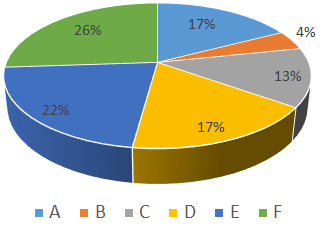
\includegraphics[scale = 0.8]{roleta.png}
\end{figure}

Observa-se que os individuos com maior probabilidade de seleção, ocupam uma área maior da roleta. A probabilidade de seleção de cada indivíduo da população é distribuída em intervalos conforme a figura \ref{fig:ditrib}

\begin{figure}[H]
\label{fig:ditrib}
  \caption{Distribuição.}
  \centering
    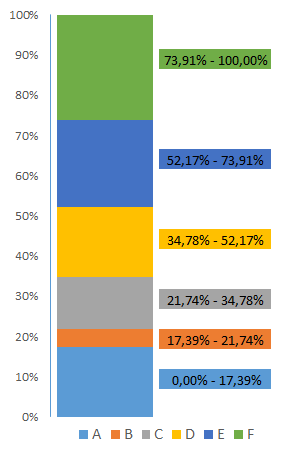
\includegraphics[scale = 1]{roleta_dist2.png}
\end{figure}

A partir dessa distribuição, um número randômico dentro do intervalo [0.00\%; 100.00\%] é gerado. Dentro os intervalos de distribuição da roleta, escolhe-se o cromossomo cujo intervalo o número gerado pertencer. O procedimento é repetido n vezes onde n é o tamanho da população.

\subsubsection{Torneio}
O método de seleção baseada em um torneio consiste em selecionar uma série de indivíduos da população para competições diretas. Os cromossomos competem diretamente, tendo como critério a função de avaliação de cada um. O cromossomo com melhor avaliação na competição é escolhido como pai. Um parâmetro para o torneio é definir o número de participantes por competição (k).
Em um exemplo de AG tem-se a seguinte população, composta por 8 indivíduos:

\begin{table}[H]
\label{tab:popinfo}
\caption{Exemplo de população}
\centering
\begin{tabular}{cc}
\toprule
Indivíduo & Avaliação\\
\midrule
A & 10\\
B & 5\\
C & 9\\
D & 1\\
E & 3\\
F & 7\\
G & 6\\
H & 2\\
\bottomrule
\end{tabular}
\end{table}

Para um critério k com valor igual a 2, serão selecionados aleatoriamente oito duplas. De cada dupla será reservado o indivíduo com função de avaliação superior.

\begin{figure}[H]
\label{fig:torneio}
  \caption{Exemplo de torneio.}
  \centering
    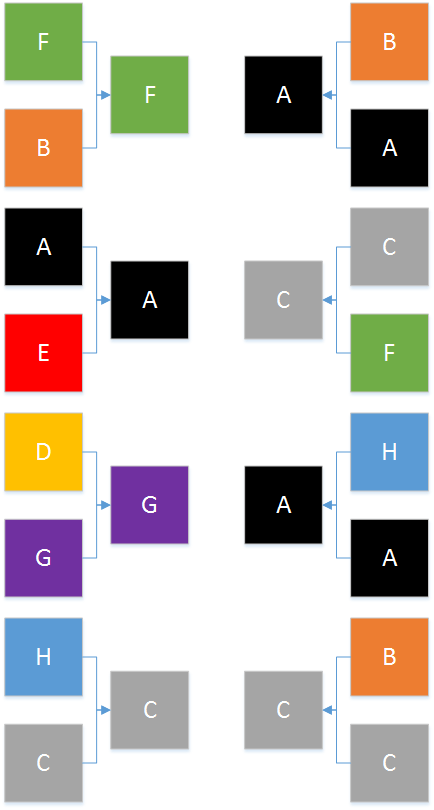
\includegraphics[scale = 0.5]{torneio.png}
\end{figure}

A partir dos indivíduos selecionados por torneio, é que se efetua o processo de cruzamento.

\subsection{Cruzamento (Crossover)}
Crossover é um operador genético usado para reprogramar a configuração de um cromossomo de uma geração para a próxima. Este operador é análogo à reprodução biológica de forma a promover a recombinação genética de duas ou mais soluções progenitoras e consequentemente gerando uma solução descendente. Existem diferentes técnicas de recombinação: com um ponto, com dois pontos,"corta e emenda", uniforme, metade uniforme, com três progenitores, cromossomos ordenados, tendenciosa, entre outras.

\subsubsection{Crossover de um ponto}
Para a aplicação foi utilizada a ténica de recombinação de um ponto. Nesta técnica um único ponto para recombinação é selecionado randomicamente para os cromossomos progenitores. Todos os genes a partir deste ponto são trocados entre os cromossomos. Os organismos resultantes são os filhos. A figura \ref{fig:c1p} ilustra um cruzamento de um ponto.

\begin{figure}[H]
\label{fig:c1p}
  \caption{Cruzamento de um ponto.}
  \centering
    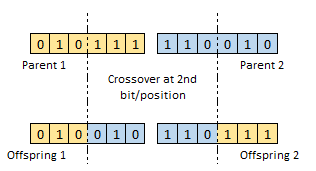
\includegraphics[scale = 0.9]{crossover_onepoint.png}
\end{figure}

Entretanto existe a possibilidade de os pais não realizarem a recombinação. Isto ocorre porque existe uma probabilidade de cruzamento (Pc) a ser considerada inicialmente. Um valor de Pc é definido nas configurações do AG antes do algoritmo ser iniciado. Para cada cromossomo parental é gerado um valor randômico (random) variando entre [0\%; 100\%]. Se a variável random possuir um valor menor ou igual ao valor de Pc, o cruzamento é efetuado. Caso contrário, os individuos não efetuam o cruzemento mantendo suas características para a próxima geração.

\subsection{Mutação}
A mutação é um operador genético utilizado para manter a diversidade gênica de uma geração de cromossomos para a próxima. É análoga à mutação presente nos sistemas biológicos. Este operador pode alterar um ou mais genes de um cromossomo. De maneira semelhante à etapa de cruzamento, a mutação possui uma probabilidade associada (Pm), que define a chance de tal processo ocorrer em um determinado momento. Um variável randômica, pertencente ao intervalo [0\%; 100\%], é gerada. Se o valor dessa variável for inferior ou igual à Pm, a mutação ocorre. Se for superior, a operação não é realizada e o cromossomo mantém suas características sem alterações.
Existem diferentes tipos de mutação: inversão de um único bit, inversão de todos os bits do cromossomo, por limites, não uniforme, uniforme, gaussiana. Para a aplicação optou-se pelo método de inversão de um único bit.

\begin{figure}[H]
\label{fig:mut}
  \caption{Mutação: inversão de um único bit}
  \centering
    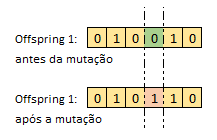
\includegraphics[scale = 0.9]{mutation.png}
\end{figure}

%------------------------------------------------

\section{Resultados}
Para a aplicação foi elaborado um formulário (\ref {fig:userview}) que possibilita ao usuário configurar os seguintes parâmetros da aplicação:
\begin{enumerate}
\item Características do algoritmo genético:
\begin{enumerate}
\item tamanho da população;
\item número de gerações;
\item probabilidade de cruzamento;
\item probabilidade de mutação.
\end{enumerate}
\item Características do cromossomo:
\begin{enumerate}
\item valor mínimo;
\item valor máximo;
\item granularidade ou resolução.
\end{enumerate}
\end{enumerate}

\begin{figure}[H]
\label{fig:userview}
  \caption{Tela de configuração do AG.}
  \centering
    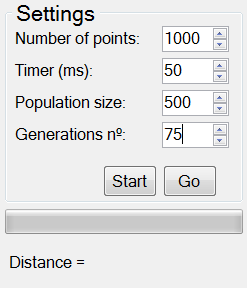
\includegraphics[scale = 0.45]{user_view.png}
\end{figure}

Ao inicializar o algoritmo genético, um outro formulário é criado, contendo dois objetos gráficos. O primeiro objeto é um gráfico bidimensional contendo a função (\ref{eq:probfunc}) proposta pelo problema. O eixo das abcissas e o eixo das ordenadas sao compostos, respectivamente, pelo valores do domínio do problema e pelo valor que a função admite para cada um desses valores (x, f(x)). Assim que a população é inicializada, os seus individuos são adicionados ao gráfico. Cada indivíduo é representado por um ponto cuja coordenada é (xn, f(xn) onde xn é o valor que o n-ésimo cromossomo possui. 

\begin{figure}[H]
\label{fig:graphicview}
  \caption{Gráfico do AG.}
  \centering
    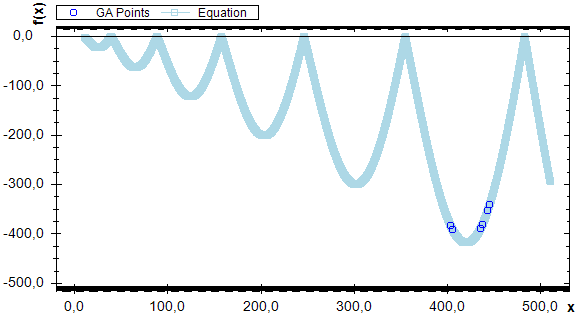
\includegraphics[scale = 0.47]{genetic_algorithm_plot.png}
\end{figure}

O outro objeto é um gráfico de performance do AG. Para cada geração (eixo x) é adicionado os valores médio e máximo da população.

\begin{figure}[H]
\label{fig:graphicview}
  \caption{Curva de performance.}
  \centering
    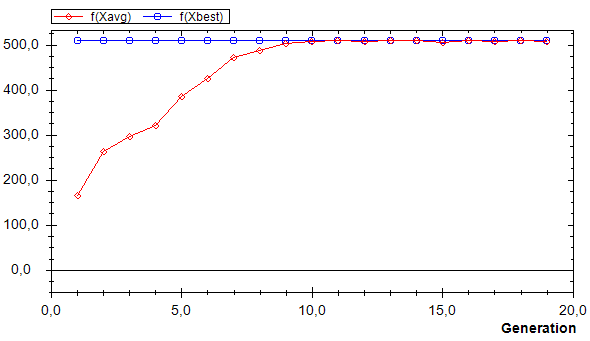
\includegraphics[scale = 0.47]{performance_curve.png}
\end{figure}

Para realizar uma análise mais detalhada do problema foi desenvolvido um outro módulo para a aplicação. Neste módulo o usuário determina os parâmetros do AG (Tamanho da população, número de gerações, probabilidade de cruzamento, probabilidade de mutação, limites de valores, resolução do cromossomo) e  o número de simulações para resolver o problema. Para cada simulação algumas informações como a melhor solução, média e desvio padrão populacional, são salvas em uma planilha. Com este módulo foi realizado os seguintes testes: Foram efetuadas 100 repetições do processamento do AG do problema, para diferentes números de gerações: 4, 8, 12, 16, 20 e 50.

\begin{table}[H]
\label{tab:popinfo}
\caption{Distribuição das probabilidades (seleção e acumulada)}
\centering
\begin{tabular}{ccc}
\toprule
PS & Tamanho da população & 50\\
Pc & Probabilidade de Cruzamento & 60\%\\
Pm & Probabilidade de Mutação & 1\%\\
Rmin & Limite mínimo & 0\\
Rmax & Limite máximo & 512\\
G & Resolução & 1\\
NR & Número de repetições & 100\\
\bottomrule
\end{tabular}
\end{table}

Após os testes, foram separados o melhor cromossomo e o desvio padrão entre as repetições para uma das diferentes condições de números de gerações do AG.

\begin{figure}[H]
\label{fig:t1}
  \caption{Avaliação do melhor cromossomo.}
  \centering
    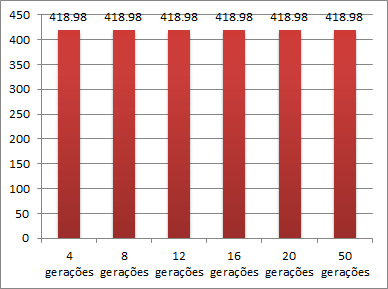
\includegraphics[scale = 0.7]{test_aval1.png}
\end{figure}

\begin{figure}[H]
\label{fig:t2}
  \caption{Desvio padrão populacional.}
  \centering
    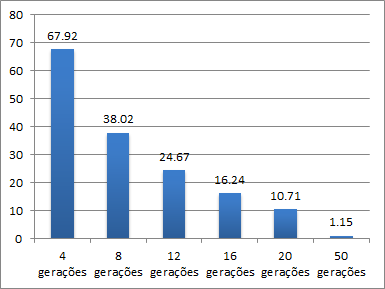
\includegraphics[scale = 0.7]{test_aval2.png}
\end{figure}
%------------------------------------------------

\section{Discussion}
Foi possível analisar em (\ref{fig:t1}) que com apenas 4 gerações o AG foi capaz de encontrar a melhor solução para o problema, haja visto que as repetições para 8, 12, 16, 20 e 50 números de gerações encontraram a mesma solução. Com relação ao desvio padrão populacional, pode-se concluir que quanto maior for o número de gerações do AG, menor será o desvio padrão da sua população. A medida que os processos de seleção e reprodução acontecem, a população elimina os indivíduos de menor avaliação em detrito dos de melhor avaliação. 
%----------------------------------------------------------------------------------------
%	REFERENCE LIST
%----------------------------------------------------------------------------------------

\begin{thebibliography}{99} % Bibliography - this is intentionally simple in this template

\bibitem[Linden, 2006]{Linden:2006dg}
Linden, R. (2006).
\newblock Algoritmos Genéticos - Uma importante ferramenta da Inteligência Computacional.
 
\end{thebibliography}

%----------------------------------------------------------------------------------------

\end{multicols}

\end{document}